\documentclass[journal,12pt,twocolumn]{IEEEtran}

\usepackage{setspace}
\usepackage{gensymb}
\singlespacing
\usepackage[cmex10]{amsmath}

\usepackage{amsthm}

\usepackage{mathrsfs}
\usepackage{txfonts}
\usepackage{stfloats}
\usepackage{bm}
\usepackage{cite}
\usepackage{cases}
\usepackage{subfig}

\usepackage{longtable}
\usepackage{multirow}

\usepackage{enumitem}
\usepackage{mathtools}
\usepackage{steinmetz}
\usepackage{tikz}
\usepackage{circuitikz}
\usepackage{verbatim}
\usepackage{tfrupee}
\usepackage[breaklinks=true]{hyperref}
\usepackage{graphicx}
\usepackage{tkz-euclide}

\usetikzlibrary{calc,math}
\usepackage{listings}
    \usepackage{color}                                            %%
    \usepackage{array}                                            %%
    \usepackage{longtable}                                        %%
    \usepackage{calc}                                             %%
    \usepackage{multirow}                                         %%
    \usepackage{hhline}                                           %%
    \usepackage{ifthen}                                           %%
    \usepackage{lscape}     
\usepackage{multicol}
\usepackage{chngcntr}

\DeclareMathOperator*{\Res}{Res}

\renewcommand\thesection{\arabic{section}}
\renewcommand\thesubsection{\thesection.\arabic{subsection}}
\renewcommand\thesubsubsection{\thesubsection.\arabic{subsubsection}}

\renewcommand\thesectiondis{\arabic{section}}
\renewcommand\thesubsectiondis{\thesectiondis.\arabic{subsection}}
\renewcommand\thesubsubsectiondis{\thesubsectiondis.\arabic{subsubsection}}

\newtheorem{theorem}{Theorem}
\hyphenation{op-tical net-works semi-conduc-tor}
\def\inputGnumericTable{}                                 %%

\lstset{
%language=C,
frame=single, 
breaklines=true,
columns=fullflexible
}
\begin{document}

\newcommand{\BEQA}{\begin{eqnarray}}
\newcommand{\EEQA}{\end{eqnarray}}
\newcommand{\define}{\stackrel{\triangle}{=}}
\bibliographystyle{IEEEtran}
\raggedbottom
\setlength{\parindent}{0pt}
\providecommand{\mbf}{\mathbf}
\providecommand{\pr}[1]{\ensuremath{\Pr\left(#1\right)}}
\providecommand{\qfunc}[1]{\ensuremath{Q\left(#1\right)}}
\providecommand{\sbrak}[1]{\ensuremath{{}\left[#1\right]}}
\providecommand{\lsbrak}[1]{\ensuremath{{}\left[#1\right.}}
\providecommand{\rsbrak}[1]{\ensuremath{{}\left.#1\right]}}
\providecommand{\brak}[1]{\ensuremath{\left(#1\right)}}
\providecommand{\lbrak}[1]{\ensuremath{\left(#1\right.}}
\providecommand{\rbrak}[1]{\ensuremath{\left.#1\right)}}
\providecommand{\cbrak}[1]{\ensuremath{\left\{#1\right\}}}
\providecommand{\lcbrak}[1]{\ensuremath{\left\{#1\right.}}
\providecommand{\rcbrak}[1]{\ensuremath{\left.#1\right\}}}
\DeclarePairedDelimiter\abs{\lvert}{\rvert}
\DeclarePairedDelimiter\norm{\lVert}{\rVert}
\theoremstyle{remark}
\newtheorem{rem}{Remark}
\newcommand{\sgn}{\mathop{\mathrm{sgn}}}
\providecommand{\abs}[1]{\vert#1\vert}
\providecommand{\res}[1]{\Res\displaylimits_{#1}} 
\providecommand{\norm}[1]{\lVert#1\rVert}
%\providecommand{\norm}[1]{\lVert#1\rVert}
\providecommand{\mtx}[1]{\mathbf{#1}}
\providecommand{\mean}[1]{E[ #1 ]}
\providecommand{\fourier}{\overset{\mathcal{F}}{ \rightleftharpoons}}
%\providecommand{\hilbert}{\overset{\mathcal{H}}{ \rightleftharpoons}}
\providecommand{\system}{\overset{\mathcal{H}}{ \longleftrightarrow}}
	%\newcommand{\solution}[2]{\textbf{Solution:}{#1}}
\newcommand{\solution}{\noindent \textbf{Solution: }}
\newcommand{\cosec}{\,\text{cosec}\,}
\providecommand{\dec}[2]{\ensuremath{\overset{#1}{\underset{#2}{\gtrless}}}}
\newcommand{\myvec}[1]{\ensuremath{\begin{pmatrix}#1\end{pmatrix}}}
\newcommand{\mydet}[1]{\ensuremath{\begin{vmatrix}#1\end{vmatrix}}}
\newtheorem{definition}{Definition}
\numberwithin{equation}{subsection}
\newtheorem{corollary}{Corollary}[theorem]
\makeatletter
\@addtoreset{figure}{problem}
\makeatother
\let\StandardTheFigure\thefigure
\let\vec\mathbf
\renewcommand{\thefigure}{\theproblem}
\def\putbox#1#2#3{\makebox[0in][l]{\makebox[#1][l]{}\raisebox{\baselineskip}[0in][0in]{\raisebox{#2}[0in][0in]{#3}}}}
     \def\rightbox#1{\makebox[0in][r]{#1}}
     \def\centbox#1{\makebox[0in]{#1}}
     \def\topbox#1{\raisebox{-\baselineskip}[0in][0in]{#1}}
     \def\midbox#1{\raisebox{-0.5\baselineskip}[0in][0in]{#1}}
\vspace{3cm}
\title{GATE Assignment 4}
\author{Digjoy Nandi - AI20BTECH11007}
\maketitle
\newpage
\bigskip
\renewcommand{\thefigure}{\theenumi}
\renewcommand{\thetable}{\theenumi}

%
Download all latex codes from 
%
\begin{lstlisting}
https://github.com/Digjoy12/Signal-Processing/blob/main/Quiz_2/main.tex
\end{lstlisting}
\section*{\textbf{Problem}}
\textbf{(GATE-EC 1999- Q 1.18)} A signal x(t) has a Fourier transform x($\omega$). If x(t) is a real and odd function of t, then x($\omega$) is
\begin{enumerate}[label=(\alph*)]
    \item a real and even function of $\omega$
    \item an imaginary and odd function of $\omega$
    \item an imaginary and even function of $\omega$
    \item a real and odd function of $\omega$
\end{enumerate}
\section*{\textbf{Solution}}
\begin{definition}{\textbf{(Even function)}}.
 For a real-valued function f(x) is even function when,
 \begin{equation}
     f(-x) = f(x)
 \end{equation}
 for all values of x in the domain of f.
\end{definition}
\begin{definition}{\textbf{(Odd function)}}.
 For a real-valued function f(x) is odd function when,
 \begin{equation}
     f(-x) = -f(x)
 \end{equation}
 for all values of x in the domain of f.
\end{definition}
\begin{corollary}\label{0.1}
The product of two odd function is even.\\
Let f(x) and g(x) be two odd function, then
\begin{align}
    f(x)g(x) = -f(x)-g(x) = f(x)g(x)
\end{align}
\end{corollary}
\begin{corollary}\label{0.2}
The product of one odd and one even function is odd.\\
Let f(x) be an even and g(x) be an odd function, then
\begin{align}
    f(x)g(x) = f(x)-g(x) = -f(x)g(x)
\end{align}
\end{corollary}

The Fourier transform of real x(t) is given by
\begin{align}
    \mathcal{F}[f(x)] &= \cfrac{1}{\sqrt{2\pi}}\displaystyle\int\limits_{-\infty}^{\infty} f(x)\exp{(-i\omega x)}dx\\
    &= \cfrac{1}{\sqrt{2\pi}}\displaystyle\int\limits_{-\infty}^{\infty} f(x)(\cos{(\omega x)} - i\sin{(\omega x)})dx\\
    &= \cfrac{1}{\sqrt{2\pi}}\displaystyle\int\limits_{-\infty}^{\infty} f(x)\cos{(\omega x)}dx -\nonumber \\ 
    &\text{ }\cfrac{i}{\sqrt{2\pi}}\displaystyle\int\limits_{-\infty}^{\infty} f(x)\sin{(\omega x)}dx \label{0.0.7}
\end{align}
Here, \\
$\cos{(\omega x)}$ is even function and f(x) is an odd function, therefore using (\ref{0.1}),
\begin{align}
    f(x)\cos{(\omega x)} \text{ is an odd function.}
\end{align}
Again,\\
$\sin{(\omega x)}$ is odd function and f(x) is an odd function, therefore using (\ref{0.2}),
\begin{align}
   f(x)\sin{(\omega x)} \text{ is an even function} 
\end{align}
Now, equation (\ref{0.0.7}) can be written as,
\begin{align}
    \mathcal{F}[f(x)] &= \cfrac{2i}{\sqrt{2\pi}}\displaystyle\int\limits_{-\infty}^{\infty} f(x)\sin{(\omega x)}dx\\
    &= i\sqrt{\cfrac{2}{\pi}}\displaystyle\int\limits_{-\infty}^{\infty} f(x)\sin{(\omega x)}dx
\end{align}
Therefore, Fourier transform of real odd function is \textbf{imaginary}.\\

Now,
The Fourier transform of an odd function is
\begin{align}
    \mathcal{F}[f(x)] &= \cfrac{1}{\sqrt{2\pi}}\displaystyle\int\limits_{-\infty}^{\infty} f(x)\exp{(-i\omega x)}dx
\end{align}
Substituting f(−x) for f(x) yields:
\begin{align}
    \mathcal{F}[f(x)] &= \cfrac{1}{\sqrt{2\pi}}\displaystyle\int\limits_{-\infty}^{\infty} f(-x)\exp{(-i\omega x)}dx    
\end{align}
Substituting u for −x and −du for dx yields:
\begin{align}
    \mathcal{F}[f(x)] &= \cfrac{1}{\sqrt{2\pi}}\displaystyle\int\limits_{u=\infty}^{u=-\infty} -f(x)\exp{(-i\omega (-x))}dx\\
    &= \cfrac{1}{\sqrt{2\pi}}\displaystyle\int\limits_{-\infty}^{\infty} f(x)\exp{(-i\omega (-x))}dx\\
    &= \mathcal{F}(-x)
\end{align}
Hence,  Fourier transform of real odd function is \textbf{odd}.\\
Hence, \textbf{the correct option is (b)}.
\begin{comment}
\begin{figure}[!ht]
\centering
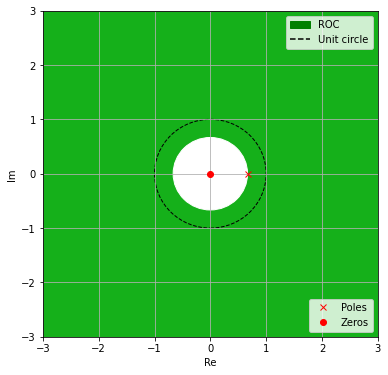
\includegraphics[width=\columnwidth]{pole_plot.png}
\caption{ROC for H(z)}
\end{figure}
\end{comment}


\end{document}
